%%%
% $Autor: Malena Wilken $
% $Date: 2025-01-29 $
% $File: IoT Introduction.tex $
% $Version: 1 $
%
% English Version C:\Users\malen\Documents\2025\Praxissemester\Ecosensors
%%%
\chapter{Introduction to IoT System for EcoSensors}
Ecosensors \ref{fig:Ecosensors} is a weather station designed to collect environmental data using a range of sensors, including temperature, humidity, pressure, and CO$_{2}$ sensors. 
The collected data is transmitted to a cloud platform, where it can be accessed by both customers and the company for monitoring and analysis purposes.
The Hypatia Board, a ESP32 controlled Board designed by the company, supports data transmission and reception via WiFi, Bluetooth Low Energy (BLE), Sigfox, and LoRaWAN.
To enable both clients and internal users to verify IoT connectivity, a set of simple test codes and a corresponding IoT manual are provided. The following section outlines the use of these codes and explains the underlying IoT communication systems. To use the test examples, a Hypatia board is required, and the Arduino IDE must be installed. More information about compatible devices and installation instructions for the Arduino IDE can be found at: https://www.arduino.cc/en/software.

\begin{figure}[H]
	\centering
	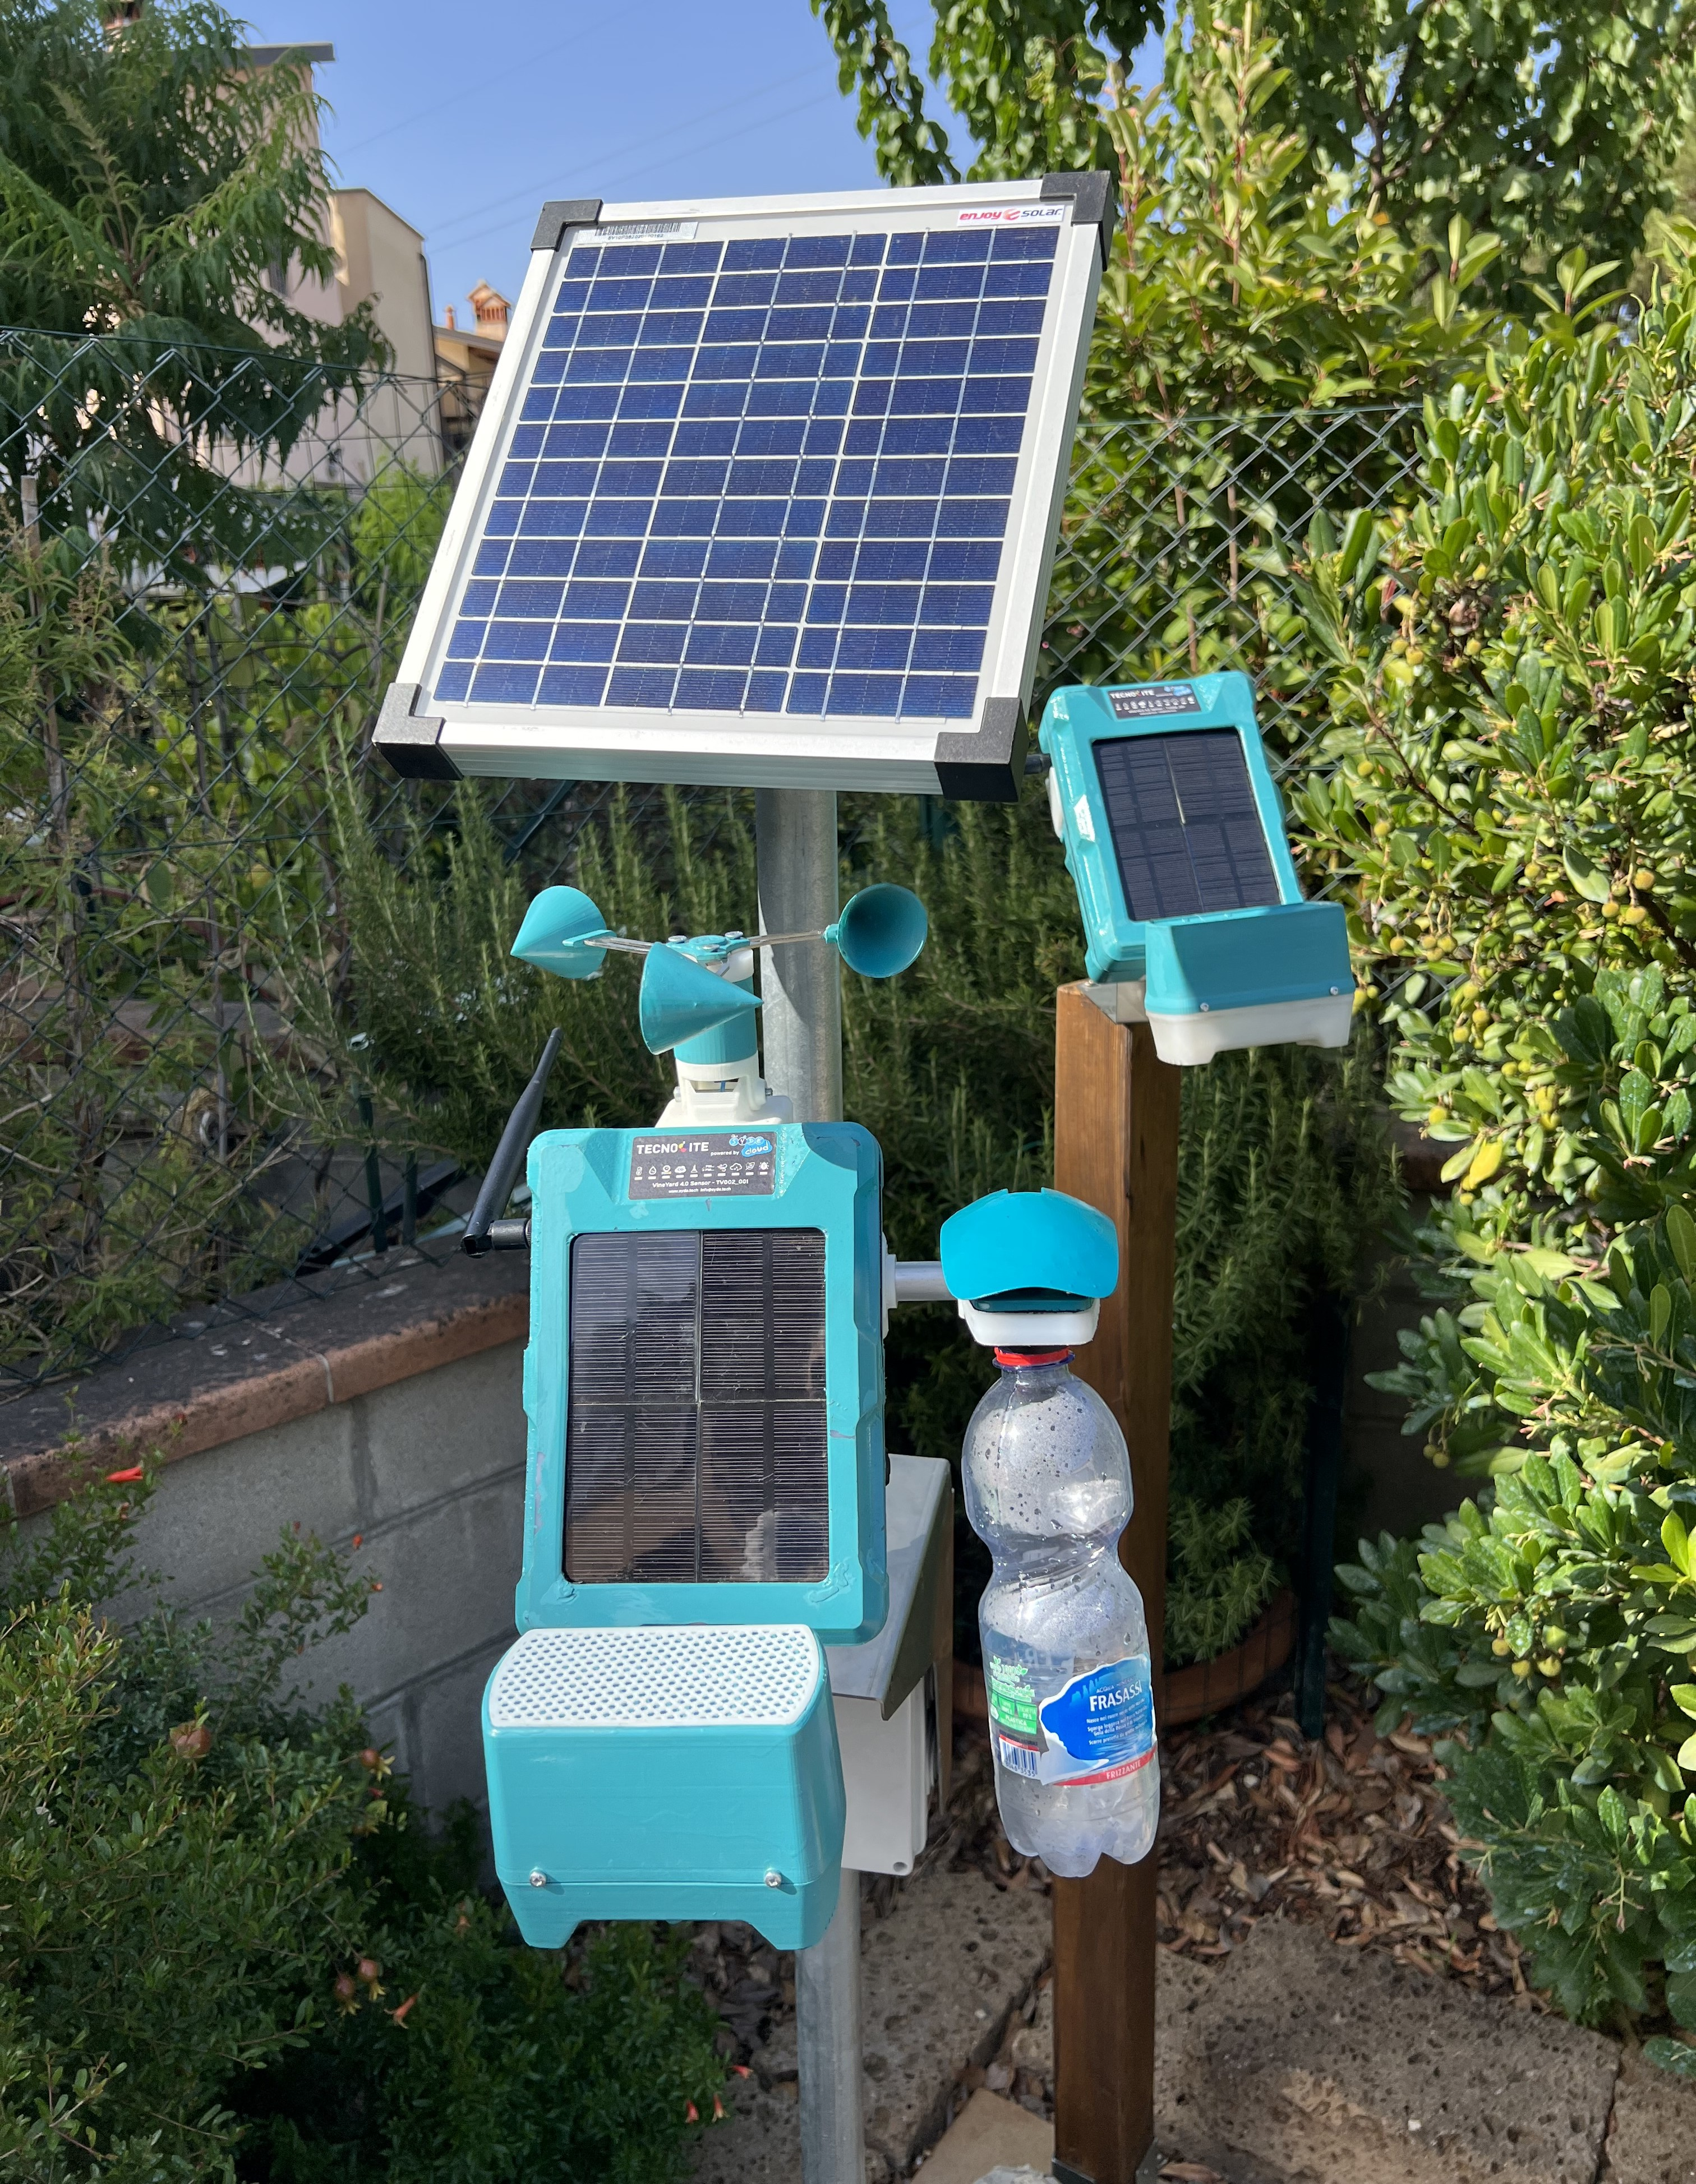
\includegraphics[width=0.4\linewidth]{../../../Images/Syde/Ecosensors}
	\caption[Ecosensors Agriculture 4.0]{Ecosensors Agriculture 4.0}
	\label{fig:Ecosensors}
\end{figure}
